\documentclass{article}
\usepackage[margin=10mm,paperwidth=230mm,paperheight=90mm]{geometry}
\usepackage{amsmath,tikz}
\usetikzlibrary{arrows.meta,positioning,calc}
\pagestyle{empty}
\begin{document}
\centering
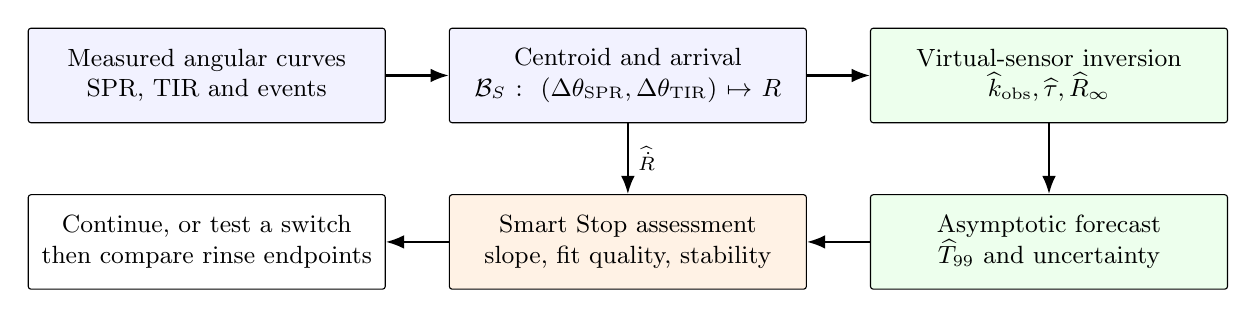
\begin{tikzpicture}[>=Latex,font=\small,
 box/.style={draw,rounded corners=1pt,align=center,minimum height=12mm,text width=43mm},
 link/.style={->,thick}]
\node[box,fill=blue!5] (input) {Measured angular curves\\SPR, TIR and events};
\node[box,right=8mm of input,fill=blue!5] (clean) {Centroid and arrival\\$\mathcal B_S:\ (\Delta\theta_{\rm SPR},\Delta\theta_{\rm TIR})\mapsto R$};
\node[box,right=8mm of clean,fill=green!7] (inverse) {Virtual-sensor inversion\\$\widehat k_{\rm obs},\widehat\tau,\widehat R_\infty$};
\node[box,below=9mm of inverse,fill=green!7] (forecast) {Asymptotic forecast\\$\widehat T_{99}$ and uncertainty};
\node[box,left=8mm of forecast,fill=orange!10] (gate) {Smart Stop assessment\\slope, fit quality, stability};
\node[box,left=8mm of gate] (outcome) {Continue, or test a switch\\then compare rinse endpoints};
\draw[link] (input)--(clean);\draw[link] (clean)--(inverse);
\draw[link] (inverse)--(forecast);\draw[link] (forecast)--(gate);
\draw[link] (clean)--node[right,font=\scriptsize] {$\widehat{\dot R}$} (gate);
\draw[link] (gate)--(outcome);
\end{tikzpicture}
\end{document}
